\documentclass[12pt,a4paper]{article}

% Input and language
\usepackage[brazilian]{babel}
\usepackage[utf8]{inputenc}

% Fonts
\usepackage[scaled]{helvet}
\renewcommand\familydefault{\sfdefault} 
\usepackage[T1]{fontenc}
\usepackage{microtype}
\usepackage{inconsolata}    % monospaced font

% Spacings and floats
\usepackage{geometry}
\addtolength{\topmargin}{-2cm}
\addtolength{\textheight}{4cm}
\usepackage{float}
\usepackage{booktabs}
\usepackage{enumitem}
\renewcommand{\theenumi}{\alph{enumi}}
\setlist{noitemsep,leftmargin=0.5cm}%$,topsep=1.5pt,parsep=1.5pt,partopsep=5pt}
\usepackage{titlesec}
\titlespacing*{\section}{0cm}{0cm}{-0.5cm}
\titlespacing*{\subsection}{-1cm}{0.4cm}{0.2cm}
\usepackage{multicol}

% Math symbols
\usepackage{amsmath,amsthm,amssymb,amsfonts}
\usepackage{braket}		% So I could use \Set

% Algoritms and Code
\usepackage[vlined,portuguese,linesnumbered,tworuled]{algorithm2e}
\usepackage[outputdir={./build}]{minted}

% Exam package
\usepackage{xsim}
\DeclareExerciseType{question}{
exercise-env      = question ,
solution-env      = answer ,
exercise-name     = questão ,
solution-name     = resposta ,
exercise-template = default ,
solution-template = default
}
\DeclareExerciseTranslations{points}{
Brazilian= pontos
}

% Images and fancy stuff
\usepackage{graphicx}
\graphicspath{{./pic/}}
\usepackage{subcaption}
\usepackage[gray,table,fixpdftex]{xcolor}
\definecolor{mylightgray}{gray}{0.95}
\definecolor{mydarkgray}{gray}{0.8}
\usepackage{tcolorbox}
\usepackage{lastpage}   
\usepackage{fancyhdr}
\fancyfoot[C]{Página \thepage\ de \pageref{LastPage}}
\renewcommand{\headrulewidth}{0pt} 
\pagestyle{fancy}

% The document
\begin{document}

% Heading
\section*{\large \centerline{\underline{Prova \color{red}{**}}}}
\section*{\normalsize \centerline{\color{red}{CODCRED - DISCIPLINA - TURMA - SEMESTRE - Prof. Diego Noble}}}
\bigskip
\begin{tabular}{lr}
	\makebox[0.8\textwidth]{Nome:\enspace\hrulefill} & \makebox[0.15\textwidth]{Nota:\enspace\hrulefill} \\
\end{tabular}

% Instructions
\begin{tcolorbox}[center title,title=\textbf{\large Instruções}, coltitle=black, colbacktitle=mydarkgray, colframe=black, colback=mylightgray]
	\begin{itemize}
	    \item A prova é individual e sem consulta a qualquer material.
	    \item Somente respostas escritas à caneta serão reavaliadas.
	    \item É proibido fazer perguntas de interpretação da prova após a leitura da mesma pelo professor.
	    \item É proibido o empréstimo de material durante a prova.
	    \item Só é permitida a entrega da prova transcorridos 20 minutos do seu início.
	    \item A prova tem valor total de \printtotalpoints.
	\end{itemize}
\end{tcolorbox}

% Questions
\begin{question}[points=2.0, subtitle=Algoritmos Gulosos]
    Você precisa definir a posição de bases de celular para cobrir \emph{todas} as casas
    que ficam ao longo de uma estrada. A estrada pode ser interpretada como um segmento
    de reta com pontas leste e oeste. Cada base de celular cobre 4 quilômetros para cada lado.
    Dê um algoritmo eficiente para encontrar todas as casas ao longo da estrada usando
    o menor número de bases possível.
\end{question}

\begin{question}[points=3.0,subtitle=Divisão-e-conquista]
	Sejam $a \geq 1$ e $b > 1$ constantes, $f(n)$ e $T(n)$ funções definidas
	sobre inteiros não-negativos, temos que:
	\begin{table}[h!]
		\centering
		$T(n) = aT(n/b) + f(n)$
	\end{table}
	\\
	Então $T(n)$ pode ser limitado assintoticamente por três regras:
	\begin{enumerate}
		\item Se $f(n) = O(n^{\log_b{a-\epsilon}})$ para uma constante $\epsilon > 0$, então $T(n)=\Theta(n^{\log_b{a}})$.
		\item Se $f(n) = \Theta(n^{\log_b{a}})$, então $T(n)=\Theta(n^{\log_b{a}}\lg n)$.
		\item Se $f(n) = \Omega(n^{\log_b{a} + \epsilon})$ para uma constante $\epsilon > 0$ e se $af(n/b) \leq cf(n)$ para uma constante $c<1$, então $T(n) = \Theta(f(n))$.
	\end{enumerate}
	Use o Método Mestre para encotrar o limite assintótico das seguintes relações de recorrência:
	\begin{multicols}{2}
		\begin{enumerate}[label=(\alph*)]
		\item $T(n)=2T(n/2)+n^4$
		\item $T(n)=T(7n/10)+n$
		\item $T(n)=16T(n/4)+n^2$
		\item $T(n)=7T(n/3)+n^2$
		\item $T(n)=7T(n/2)+n^2$
		\item $T(n)=8T(n/2)+n^3$
		\end{enumerate}
	\end{multicols}
\end{question}

\begin{question}[points=2.5, subtitle=Algoritmos Gulosos]
	Considere o problema de encontrar o troco para $n$ centavos usando o menor
	número possível de moedas. Assuma que cada moeda tem um respectivo valor inteiro.
	\begin{enumerate}[label=(\alph*)]
		\item Descreva um algoritmo guloso em pseudo-código que determina o
		troco considerando quatro valores de moedas: $25$, $10$, $5$ e $1$ centavos.
		Justifique com suas palavras porque o algoritmo encontra o troco correto
		usando o menor número de moedas possível para este conjunto de valores.
		\item Agora suponha que os valores das moedas disponíveis são um produto
		de um fator	inteiro $c>1$. Por exemplo, supondo $c=2$, temos os seguintes
		valores: $2^0$, $2^1$, $2^2$, $\ldots$, $2^k$, onde
		$k\geq1$. Mostre que o seu algoritmo também encontra o troco usando um
		número mínimo de moedas neste caso.
		\item Dê um conjunto de valores para as moedas de forma com que o seu 
		algoritmo guloso não encontre a resposta ótima. Você deve incluir necessariamente
		a moeda de $1$ centavo neste conjunto. Justifique a resposta.
	\end{enumerate}
\end{question}

\begin{question}[points=3.0]
	Considere o seguinte código abaixo em Java:
		\inputminted[
			fontfamily=tt,
			%fontsize=\small,
			frame=lines,
			framerule=0.4pt,
			framesep=2mm,
			tabsize=4,
			obeytabs=true,
			samepage=true,
			showspaces=false,
			showtabs=false,
			style=bw,
			texcl=false,
			linenos,
			highlightlines={12},
			texcomments=true
			]
		{java}{./code/TSP.java}
	A classe \texttt{Point} modela pontos $(x,y)$ em um sistema cartersiano e tem um método de classe para calcular a distância entre dois pontos.
	A classe \texttt{TSP} cria alguns pontos aleatórios como demonstração e tem um método \texttt{tspCertf}.
\end{question}

\newpage

\begin{question}[points=2, bonus-points=0.5]
	O pseudo-código abaixo para serve para realizar a busca em largura em grafo.
	\begin{algorithm}
		\SetKwData{s}{s}
		\SetKwFunction{enq}{ENQUEUE}
		\SetKwFunction{deq}{DEQUEUE}
		\SetKwData{G}{G}
		\SetKwData{V}{V}
		\SetKwData{E}{E}
		\SetKwData{Q}{Q}
		\small
		\Entrada{Um grafo $\G=(\V,\E)$ e um vértice origem $\s \in \V$.}
		%\Resultado{Tabela \textit{cache} com os pesos ótimos para cada subproblema.}
		\Inicio{
			\ParaCada{$v \in \V, v \neq \s$}{
				$v.dist \leftarrow \infty$\;
				$v.visited \leftarrow \mathtt{false}$\;
			}
			$\s.dist \leftarrow 0$\;
			$\s.visited \leftarrow \mathtt{true}$\;
			$\Q \leftarrow \emptyset$\; 
			$\Q.\enq(\s)$\;
			\Enqto{$\Q \neq \emptyset$}{
				$u \leftarrow \Q.\deq()$\;
				\ParaCada{$v \in \G.Adj[u]$}{
					\Se{$v.visited == \mathtt{false}$ }{
						$v.visited \leftarrow \mathtt{true}$\;
						$v.dist \leftarrow u.dist + 1$\;
						$\Q.\enq(v)$\;
					}
				}
				$u.visited \leftarrow \mathtt{true}$\;
			}
		}
	\end{algorithm}
	\begin{figure}[h]
		\centering
		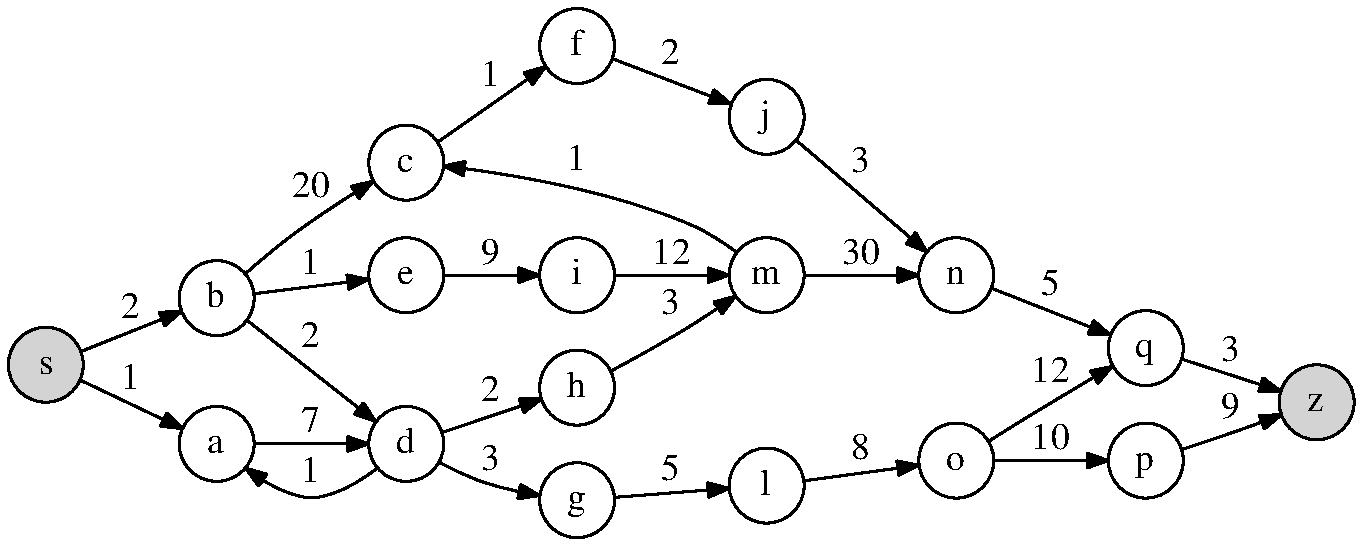
\includegraphics[scale=0.6]{smallest.pdf}
        \caption{Um grafo.}
	\end{figure}
\end{question}

\begin{question}
    Algumas afirmações abaixo são verdadeiras e outras são falsas:
    \begin{enumerate}[label=(\alph*)]
        \item Morbi ac imperdiet nisi. Interdum et malesuada fames ac ante ipsum primis in faucibus. Donec lobortis magna nibh, a consequat libero convallis sit amet.
        \item Phasellus tellus libero, gravida tempor fringilla et, viverra ut sem. Nunc et nulla neque. 
        \item Lisque id eros pellentesque, fringilla neque at, ultricies lorem.
        \item Integer a efficitur leo. 
        \item Sed facilisis tempus tellus sit amet elementum. 
    \end{enumerate}
    Preencha a tabela abaixo com \textbf{V} para as respectivas  afirmações verdadeiras e \textbf{F} nas respectivas afirmações falsas.
    \begin{table}[h]
        \centering
        \begin{tabular}{l|c|c|c|c|c|}
            \toprule
            Afirmação & a & b & c & d & e \\
            \midrule
            Resposta &  &  &  &  &  \\
            \bottomrule
        \end{tabular}
    \end{table}
\end{question}
\begin{answer}[print=true]
    \begin{table}[h]
        \centering
        \begin{tabular}{l|c|c|c|c|c|}
            \toprule
            Afirmação & a & b & c & d & e \\
            \midrule
            Resposta & V & V & F & V & V \\
            \bottomrule
        \end{tabular}
    \end{table}
\end{answer}

\end{document}